% Jacob Neumann

% DOCUMENT CLASS AND PACKAGE USE
    \documentclass[aspectratio=169, handout]{beamer}

    % Establish the colorlambda boolean, to control whether the lambda is solid color (true), or the same as the picture (false)
    \newif\ifcolorlambda
    \colorlambdafalse % DEFAULT: false

    % Use auxcolor for syntax highlighting
    \newif\ifuseaux
    \useauxfalse % DEFAULT: false

    % Color settings
    \useauxtrue

    \newcommand{\auxColor}{B66F2D}     % the color of note boxes and stuff
    \newcommand{\presentColor}{929292} % the primary color of the slide borders
    \newcommand{\bgColor}{f0e9e1}      % the color of the background of the slide
    \newcommand{\darkBg}{8b98ad}
    \newcommand{\lambdaColor}{\auxColor}

    \colorlambdatrue

    \usepackage{comment} % comment blocks
    \usepackage{soul} % strikethrough
    \usepackage{listings} % code
    \usepackage{makecell}

    \setbeamertemplate{itemize items}[circle]
    % \setbeameroption{show notes on second screen=right}

    \usepackage{lectureSlides}
    %%%%%%%%%%%%%%%%%%%%%%%%%%%%%%%%%%%%%%%%%| <----- Don't make the title any longer than this
    \title{Imperative Programming} % TODO
    \subtitle{Breaking all the rules} % TODO
    \date{27 July 2023} % TODO
    \author{Brandon Wu} % TODO

    \graphicspath{ {./img/} }

    \definecolor{boxColor}{HTML}{fce1c0}
    \definecolor{highlightColor}{HTML}{faf89d}

    \usetikzlibrary {shapes.symbols}
    \usetikzlibrary {calc}
    \tikzset{
      every path/.style={line width=0.25mm},
      box/.style={
        rectangle, draw=black, inner sep=0.4cm, thick,
        minimum height=1cm,
        fill=boxColor,
        font=\large,
      },
      hlbox/.style={
        rectangle, draw=black, inner sep=0.4cm, thick,
        minimum height=1cm,
        fill=highlightColor,
      }
    }

    \newcommand{\topthing}[2]{
      \begin{minipage}[t][#1][t]{\textwidth}
        \vspace{\fill}
        #2
        \vspace{\fill}
      \end{minipage}
    }

    % DONT FORGET TO PUT [fragile] on frames with codeblocks, specs, etc.
        %\begin{frame}[fragile]
        %\begin{codeblock}
        %fun fact 0 = 1
        %  | fact n = n * fact(n-1)
        %\end{codeblock}
        %\end{frame}

    % INCLUDING codefile:
        % 1. In some file under code/NN (where NN is the lecture id num), include:
    %       (* FRAGMENT KK *)
    %           <CONTENT>
    %       (* END KK *)

    %    Remember to not put anything on the same line as the FRAGMENT or END comment, as that won't be included. KK here is some (not-zero-padded) integer. Note that you MUST have fragments 0,1,...,KK-1 defined in this manner in order for fragment KK to be properly extracted.
        %  2. On the slide where you want code fragment K
                % \smlFrag[color]{KK}
        %     where 'color' is some color string (defaults to 'white'. Don't use presentColor.
    %  3. If you want to offset the line numbers (e.g. have them start at line 5 instead of 1), use
                % \smlFragOffset[color]{KK}{5}

\begin{document}

% Make it so ./mkWeb works correctly
\ifweb
    \renewcommand{\pause}{}
\fi

\setbeamertemplate{itemize items}[circle]

% SOLID COLOR TITLE (see SETTINGS.sty)
{
\begin{frame}[plain]
    \colorlambdatrue
    \titlepage
\end{frame}
}

\menti{8916 0183}

\begin{frame}[fragile]
  \frametitle{Lesson Plan}

  \tableofcontents
\end{frame}

\sectionSlide{1}{Mutability}

\begin{frame}[fragile]
  \frametitle{On Safety}

  So far in this course, we've spent a great deal of time emphasizing the
  importance of safety in programming.

  \pause
  \vspace{\fill}

  We want to avoid footguns like mutability, which quickly leads us into
  needing to reason profusely about the entire history of our program, as well as
  introducing the possibility of messing ourselves up by causing code which worked
  previously to no longer work.

  \pause
  \vspace{\fill}

  Our solution was to simply not to play, by only dealing with \term{pure} code
  which eschewed side effects for predictable, safe behavior.
\end{frame}

\begin{frame}[fragile]
  \frametitle{On Effects}

  We've tried our best, but effects are kind of hard to get away from!

  \pause
  \vspace{\fill}

  For instance, we saw in an earlier lecture that the presence of exceptions makes
  addition no longer commutative, in general, for arbitrary expressions. We would
  like to be able to say that independent computations can be freely reordered,
  but we can't reorder these two declarations of \code{x} and \code{y}:

  \pause
  \vspace{\fill}

  \begin{codeblock}
    fun foo () =
      let
        val x = loop ()
        val y = raise Div
      in
        ()
      end
  \end{codeblock}
\end{frame}

\begin{frame}[fragile]
  \frametitle{Printing in SML}

  Relatedly, our notion of extensional equivalence is not necessarily preserved,
  either.

  \pause
  \vspace{\fill}

  We want to say that extensionally equivalent values can be freely substituted
  for each other wherever we see them. Unfortunately, there also exists
  the \code{print} function, which has type \code{string -> unit}, which
  prints a string to the outside world.

  \pause
  \vspace{\fill}

  We can't necessarily say that \code{print "hi"} and \code{()} are extensionally
  equivalent, because replacing all instances of \code{()} will definitely make
  a program with differing extensional behavior. So we need to update our
  definition of extensional equivalence, in the presence of side effects.
\end{frame}


\begin{frame}[fragile]
  \frametitle{On Reality}

  Life is cruel. Unfortunately, we live in the physical world.

  \pause
  \vspace{\fill}

  We've shyed away from it thus far, but at some point we have to be able to read
  from files, which is a side effect of its own. At some point, we need to be able
  to interface with the real world. We can't get away from reality forever.

  \pause
  \vspace{\fill}

  So what can we do, while maintaining our ability to \textit{generally} write
  safe code, and avoid the footguns of the real world?
\end{frame}

\begin{frame}[fragile]
  \frametitle{Serving Purity}

  The key term here will be that we want to \textit{avoid} footguns.

  \pause
  \vspace{\fill}

  Like many other concepts in programming, immutability and purity are concepts
  which serve our purposes -- we do not serve theirs. That means that we do
  not need to bend over backwards to achieve immutability and purity, if the
  alternative is genuinely more useful in a particular circumstance.\footnote{Worth
  noting that there \textit{are} programming languages which do achieve \textit{complete}
  purity, like Haskell, and can still do things like interface with the real world,
  paradoxically. But it's kind of complex to understand how it does so.}

  \pause
  \vspace{\fill}

  That being said, we still don't want to use mutable code all over the place, but
  we want to simply offer the \textit{option} to. The key behind immutability is
  not to forbid mutability, but to make mutability \textit{opt-in}.
\end{frame}

\begin{frame}[fragile]
  \frametitle{Opting In}

  We've seen this in several different contexts this semester. For instance, consider
  the phenomenon of \term{null pointers}, which are when values in other programming
  languages can always possibly be some unsafe \code{NULL} value.

  \pause
  \vspace{\fill}

  This is commonly known as Tony Hoare's
  {\color{blue}\href{https://www.infoq.com/presentations/Null-References-The-Billion-Dollar-Mistake-Tony-Hoare/}{"billion-dollar mistake"}}\footnote{His words, not mine.}

  \pause
  \vspace{\fill}

  Our solution to this problem has been to make \code{option}al values intentional,
  by requiring them to be explicitly used when some \code{NONE} case is necessary.
  In other words, \code{option}al values are \textit{opt-in}, in that they only
  show up when they are chosen to.

  \pause
  \vspace{\fill}

  We are going to take a similar approach with mutability.
\end{frame}

\sectionSlide{2}{Reference Cells}

\begin{frame}[fragile]
  \frametitle{A Type for Mutability}

  Similarly to how the type \code{t option} is the type of values of type \code{t},
  plus the possibility of not having such a value at all, we are going to have a
  brand new type which denotes \term{mutable storage} of values of a certain type.

  \pause
  \vspace{\fill}

  \defBox{}{The type \code{t ref}, for any type \code{t}, is the type of mutable
  references to values of type \code{t}.}

  \pause
  \vspace{\fill}

  In other words, the type \code{t ref} is the type of \textit{boxes}, which contain
  a single value of type \code{t}.

  \vspace{\fill}

  \begin{center}
    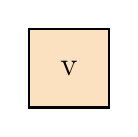
\begin{tikzpicture}
      \node[box] (N1) {\large \code{v}};
    \end{tikzpicture}
  \end{center}

  \pause
  \vspace{\fill}

  The key thing is that the contents of the box are allowed to change, as the
  program evolves!
\end{frame}

\begin{frame}[fragile]
  \frametitle{Opting Out}

  \tgs

  For anyone familiar with imperative programming, this is just a pointer to
  some mutable state. What's the difference?

  \pause
  \vspace{\fill}

  The key innovation here is that mutability is \textit{opt-in}, since we don't
  \textit{need} to use \code{ref} types unless we want to. In other words, we now
  have a \term{type-level distinction} between immutability and mutability. If we
  have a bug with some mutability going on in our code, all we need to do is look
  for the explicit places where \code{ref}s are used, rather than literally every
  assignment ever, as in an imperative language.

  \pause
  \vspace{\fill}

  This is just another example of how types will guide the structure of our programs.
\end{frame}

\begin{frame}[fragile]
  \frametitle{Mutable Primitives}

  There are a few primitives that we will use to manipulate values of \code{ref}
  type. These are the \code{ref}, \code{!}, and \code{:=} operators.

  \pause
  \vspace{\fill}

  \begin{codeblock}
    val ref : 'a -> a ref
    val !   : 'a ref -> 'a
    val :=  : 'a ref * 'a -> unit
  \end{codeblock}

  \pause
  \vspace{\fill}

  These primitives are used for creation, modification, and access for \code{ref}
  boxes.
\end{frame}

\begin{frame}[fragile]
  \frametitle{\code{ref} Creation}

  The \code{ref} function takes in a value and puts it into a mutable box.

  \pause
  \vspace{\fill}

  \begin{center}
    \begin{minipage}{0.15\textwidth}
      \centering
      \code{ref v}
    \end{minipage}
    \pause
    \begin{minipage}{0.1\textwidth}
      \centering
      $\hookrightarrow$
    \end{minipage}
    \begin{minipage}{0.15\textwidth}
      \centering
      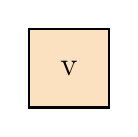
\begin{tikzpicture}
        \node[box] (N1) {\large \code{v}};
      \end{tikzpicture}
    \end{minipage}
  \end{center}

  \pause
  \vspace{\fill}

  \customBox{Key Fact}{\, The value denoted by \code{ref v} is the box itself,
  not the contents of the box!}

  \pause
  \vspace{\fill}

  In terms of what SML is doing, the act of calling the \code{ref} function
  allocates a single box, capable of storing a single value of type \code{t},
  for some type \code{t}.

  \pause
  \vspace{\fill}

  \noteBox{}{A \code{ref} box can never be empty! Because it is given an initial
  value to store inside of it, if the \code{ref} function is called at all, it
  is initially full, and there is no way to remove what's inside. No "null".}
\end{frame}

\begin{frame}[fragile]
  \frametitle{\code{ref} Creation}

  It's also worth noting that \code{ref} creation is something which occurs
  \textbf{once per call to \code{ref}}.

  \pause
  \vspace{\fill}

  Each box created by a different call to \textbf{ref} is unique, and does not
  share the same space. This means that if you want storage that is separate
  from pre-existing \code{ref}s, you should call \code{ref} again, rather than
  reuse existing ones.

  \pause
  \vspace{\fill}

  So for instance, for the following code:

  \begin{codeblock}
    val r1 = ref 1
    val r2 = ref "5"
    val r3 = ref 0
  \end{codeblock}
\end{frame}

\begin{frame}[fragile]
  \frametitle{One \code{ref}, One Box}

  \begin{center}
    \begin{minipage}[t][2.5in][t]{0.55\textwidth}
      \vspace{\fill}
      \begin{codeblock}
        val r1 = ref 1
        val r2 = ref "5"
        val r3 = ref 0
      \end{codeblock}
      \vspace{\fill}
    \end{minipage}
    \hfill\vline\hfill
    \begin{minipage}[t][2.5in][t]{0.35\textwidth}
      \centering
      {\hspace{-20pt}\color{gray} \large THE STORE}

      \vspace{\fill}
      \begin{tikzpicture}
      \end{tikzpicture}
      \vspace{\fill}
    \end{minipage}
  \end{center}
\end{frame}

\begin{frame}[fragile]
  \frametitle{One \code{ref}, One Box}

  \begin{center}
    \begin{minipage}[t][2.5in][t]{0.55\textwidth}
      \vspace{\fill}
      \begin{codeblock}
        `val r1 = ref 1`
        val r2 = ref "5"
        val r3 = ref 0
      \end{codeblock}
      \vspace{\fill}
    \end{minipage}
    \hfill\vline\hfill
    \begin{minipage}[t][2.5in][t]{0.35\textwidth}
      \centering
      {\hspace{-20pt}\color{gray} \large THE STORE}

      \vspace{\fill}
      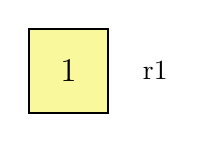
\begin{tikzpicture}
        \node[hlbox, label={[label distance=0.3cm]right:\code{r1}}] (N1) {\large \code{1}};
      \end{tikzpicture}
      \vspace{\fill}
    \end{minipage}
  \end{center}
\end{frame}

\begin{frame}[fragile]
  \frametitle{One \code{ref}, One Box}

  \begin{center}
    \begin{minipage}[t][2.5in][t]{0.55\textwidth}
      \vspace{\fill}
      \begin{codeblock}
        val r1 = ref 1
        `val r2 = ref "5"`
        val r3 = ref 0
      \end{codeblock}
      \vspace{\fill}
    \end{minipage}
    \hfill\vline\hfill
    \begin{minipage}[t][2.5in][t]{0.35\textwidth}
      \centering
      {\hspace{-20pt}\color{gray} \large THE STORE}

      \vspace{\fill}
      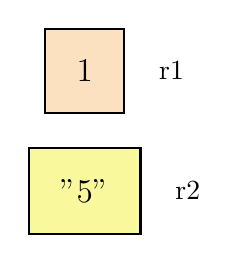
\begin{tikzpicture}
        \node[box, label={[label distance=0.3cm]right:\code{r1}}] (N1) {\code{1}};
        \node[hlbox, label={[label distance=0.3cm]right:\code{r2}}, below of=N1, node distance=0.6in] (N2) {\large \code{"5"}};
      \end{tikzpicture}
      \vspace{\fill}
    \end{minipage}
  \end{center}
\end{frame}

\begin{frame}[fragile]
  \frametitle{One \code{ref}, One Box}

  \begin{center}
    \begin{minipage}[t][2.5in][t]{0.55\textwidth}
      \vspace{\fill}
      \begin{codeblock}
        val r1 = ref 1
        val r2 = ref "5"
        `val r3 = ref 0`
      \end{codeblock}
      \vspace{\fill}
    \end{minipage}
    \hfill\vline\hfill
    \begin{minipage}[t][2.5in][t]{0.35\textwidth}
      \centering
      {\hspace{-20pt}\color{gray} \large THE STORE}

      \vspace{\fill}
      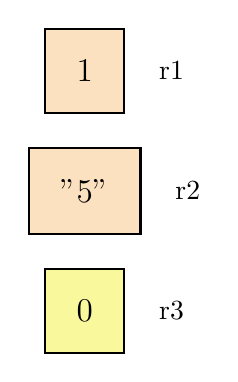
\begin{tikzpicture}
        \node[box, label={[label distance=0.3cm]right:\code{r1}}] (N1) {\code{1}};
        \node[box, label={[label distance=0.3cm]right:\code{r2}}, below of=N1, node distance=0.6in] (N2) {\code{"5"}};
        \node[hlbox, label={[label distance=0.3cm]right:\code{r3}}, below of=N2, node distance=0.6in] (N3) {\large \code{0}};
      \end{tikzpicture}
      \vspace{\fill}
    \end{minipage}
  \end{center}
\end{frame}

\begin{frame}[fragile]
  \frametitle{\code{ref} Modification}

  What if we want to change the contents of the box, though? That's where the
  \code{:=} operator\footnote{Which can be pronounced "walrus", "assignment", or "colon equals".}
  comes in, which is an infix operator of type \code{'a ref * 'a -> unit}.

  \pause
  \vspace{\fill}

  For instance, take the following code, in the context of the previous three boxes:
  \begin{codeblock}
    val () = v1 := 1
    val () = v2 := "1"
  \end{codeblock}

  \pause
  \vspace{\fill}

  Note how the \code{:=} operator returns a \code{()}, because it is strictly used
  for its side effects, and computes no meaningful values.
\end{frame}

\begin{frame}[fragile]
  \frametitle{Modifying \code{ref}s}

  \begin{center}
    \begin{minipage}[t][2.5in][t]{0.55\textwidth}
      \vspace{\fill}
      \begin{codeblock}
        val () = v1 := 2
        val () = v2 := "1"
      \end{codeblock}
      \vspace{\fill}
    \end{minipage}
    \hfill\vline\hfill
    \begin{minipage}[t][2.5in][t]{0.35\textwidth}
      \centering
      {\hspace{-20pt}\color{gray} \large THE STORE}

      \vspace{\fill}
      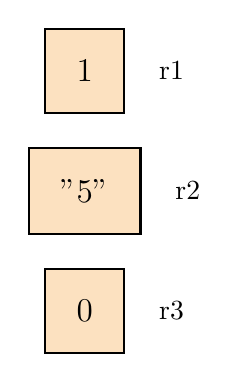
\begin{tikzpicture}
        \node[box, label={[label distance=0.3cm]right:\code{r1}}] (N1) {\code{1}};
        \node[box, label={[label distance=0.3cm]right:\code{r2}}, below of=N1, node distance=0.6in] (N2) {\code{"5"}};
        \node[box, label={[label distance=0.3cm]right:\code{r3}}, below of=N2, node distance=0.6in] (N3) {\code{0}};
      \end{tikzpicture}
      \vspace{\fill}
    \end{minipage}
  \end{center}
\end{frame}

\begin{frame}[fragile]
  \frametitle{Modifying \code{ref}s}

  \begin{center}
    \begin{minipage}[t][2.5in][t]{0.55\textwidth}
      \vspace{\fill}
      \begin{codeblock}
        `val () = v1 := 2`
        val () = v2 := "1"
      \end{codeblock}
      \vspace{\fill}
    \end{minipage}
    \hfill\vline\hfill
    \begin{minipage}[t][2.5in][t]{0.35\textwidth}
      \centering
      {\hspace{-20pt}\color{gray} \large THE STORE}

      \vspace{\fill}
      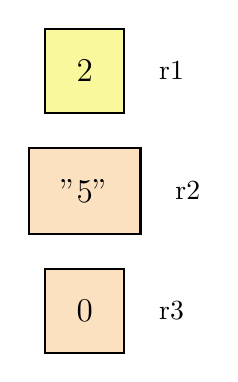
\begin{tikzpicture}
        \node[hlbox, label={[label distance=0.3cm]right:\code{r1}}] (N1) {\large \code{2}};
        \node[box, label={[label distance=0.3cm]right:\code{r2}}, below of=N1, node distance=0.6in] (N2) {\code{"5"}};
        \node[box, label={[label distance=0.3cm]right:\code{r3}}, below of=N2, node distance=0.6in] (N3) {\code{0}};
      \end{tikzpicture}
      \vspace{\fill}
    \end{minipage}
  \end{center}
\end{frame}

\begin{frame}[fragile]
  \frametitle{Modifying \code{ref}s}

  \begin{center}
    \begin{minipage}[t][2.5in][t]{0.55\textwidth}
      \vspace{\fill}
      \begin{codeblock}
        val () = v1 := 2
        `val () = v2 := "1"`
      \end{codeblock}
      \vspace{\fill}
    \end{minipage}
    \hfill\vline\hfill
    \begin{minipage}[t][2.5in][t]{0.35\textwidth}
      \centering
      {\hspace{-20pt}\color{gray} \large THE STORE}

      \vspace{\fill}
      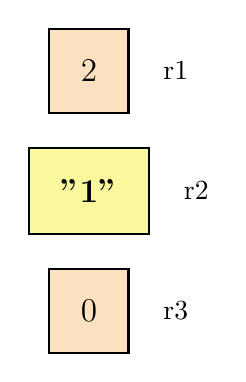
\begin{tikzpicture}
        \node[box, label={[label distance=0.3cm]right:\code{r1}}] (N1) {\code{2}};
        \node[hlbox, label={[label distance=0.3cm]right:\code{r2}}, below of=N1, node distance=0.6in] (N2) {\large \textbf{\code{"1"}}};
        \node[box, label={[label distance=0.3cm]right:\code{r3}}, below of=N2, node distance=0.6in] (N3) {\code{0}};
      \end{tikzpicture}
      \vspace{\fill}
    \end{minipage}
  \end{center}
\end{frame}

\begin{frame}[fragile]
  \frametitle{Typed Boxes}

  When we have boxes, it seems like we should be able to do anything!

  \pause
  \vspace{\fill}

  However, if our code had contained the following line, then our code
  would never have run, because it would not have type-checked:
  \begin{codeblock}
    val () = v2 := 1
  \end{codeblock}

  \pause
  \vspace{\fill}

  This is because \code{v2} is of type \code{string ref}, and
  \code{:= : 'a ref * 'a -> unit}, so it doesn't type-check!

  \pause
  \vspace{\fill}

  In principle, this is because when we make a box, it is only able to store
  values of a certain type. So we don't have complete freedom, here.
\end{frame}

\begin{frame}[fragile]
  \frametitle{\code{ref} Access}

  Finally, we have discussed how to make boxes, and how to put stuff into boxes.
  Now we need to discuss how to take things out.

  \pause
  \vspace{\fill}

  This is achieved via the \code{!} operator, pronounced as the "bang" operator,
  of type \code{'a ref -> 'a}, which simply returns whatever value is currently
  in the box.

  \pause
  \vspace{\fill}

  So in the current example:

  \begin{center}
    \begin{minipage}{0.15\textwidth}
      \centering
      \code{!v1}
    \end{minipage}
    \begin{minipage}{0.1\textwidth}
      \centering
      $+$
    \end{minipage}
    \begin{minipage}{0.15\textwidth}
      \centering
      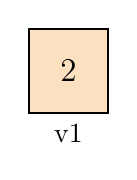
\begin{tikzpicture}
        \node[box, label=below:\code{v1}] (N1) {\code{2}};
      \end{tikzpicture}
    \end{minipage}
    \begin{minipage}{0.1\textwidth}
      \centering
      $\hookrightarrow$
    \end{minipage}
    \begin{minipage}{0.15\textwidth}
      \centering
      \code{2}
    \end{minipage}
  \end{center}

  \pause
  \vspace{\fill}

  We simply unpack the contents of the box \code{v1}, which is \code{2}.
\end{frame}

\begin{frame}[fragile]
  \frametitle{\code{ref} Access in Pattern Matching}

  Note that we can also do this \code{!} access by pattern matching.

  \pause
  \vspace{\fill}

  For instance, for the refs \code{v1 : int ref} and \code{v2 : string ref}
  that we have been working with, we could write:
  \begin{codeblock}
    case (v1, v2) of
      (ref 2, ref "1") => true
    | _ => false
  \end{codeblock}
  which would successfully return \code{true}. We might say that this kind
  of pattern matching includes an \textit{implicit deference}, because we
  access the contents of each ref without needing to call \code{!} explicitly.

  \pause
  \vspace{\fill}

  Note that this works because \code{ref} is not just a function of type
  \code{'a -> 'a ref}, it is also a constructor!
\end{frame}

\begin{frame}[fragile]
  \frametitle{Effects with Bindings}

  So far, we've been using \code{val} bindings, which don't actually bind
  anything interesting, but merely serve to evaluate some expression for
  side-effecting purposes.

  \pause
  \vspace{\fill}

  This might look something like this, for instance:
  \begin{codeblock}
    let
      val () = r := 150
    in
      e
    end
  \end{codeblock}

  if we wanted to set some \code{ref} to the value \code{150}, prior to
  evaluating some expression \code{e}.

  \pause
  \vspace{\fill}

  This is a lot to type out, though! Luckily, there's a shorthand.

\end{frame}

\begin{frame}[fragile]
  \frametitle{The Sequencing Operator}

  We can use the \code{;}, which is the \term{sequencing operator}, to
  evaluate some expressions in a sequence, while disregarding their value.

  \pause
  \vspace{\fill}

  So for instance, for the previous example, we could instead write out the
  expression \code{(r := 150; e)}. This evaluates both expressions from left-to-right
  to values, but only returns the value of the last entry. This would be extensionally
  equivalent to the previous expression.

  \pause
  \vspace{\fill}

  We can also nest these arbitrarily deep. So we could write \code{(r := 1; r :=
  5; r:= 0; 150)}\footnote{Generally, you need parentheses around the whole
  thing, whenever you have a sequence of expressions.} for the expression which
  cannot make up its mind and constantly reassigns the ref \code{r}, and then
  eventually reduces to the value \code{150}.
\end{frame}

\quizBreak{\textlangle obfuscated\textrangle}

\sectionSlide{3}{Using Refs}

\begin{frame}[fragile]
  \frametitle{Writing Imperative Code}

  Now that we know the three fundamental operators for working with \code{ref}
  cells, we can start looking at some examples of us actually using \code{ref}s.

  \pause
  \vspace{\fill}

  Now we can define some functions that we previously also could,
  but now we can do it with \code{ref}s. Let's go back to our roots. Here's \code{fact}.\footnote{Disclaimer that this is, of course,
  strictly educational, and in practice a terrible idea. You should never introduce
  mutability for the sake of mutability.}

  \pause
  \vspace{\fill}

  \begin{codeblock}
    val store = ref 1

    fun fact 0 = !store
      | fact n =
          ( store := n * (!store);
            fact (n - 1)
          )
  \end{codeblock}

  \pause
  \vspace{\fill}

  Seems legit, right?
\end{frame}

\begin{frame}[fragile]
  \frametitle{Debugging Imperative Code}

  \begin{minipage}[t][0.6in][t]{\textwidth}
  At least, it would be, if we didn't end up in the entirely predictable
  circumstance where writing imperative code ended up causing a bug.

  \pause
  \vspace{\fill}

  This \code{fact} implementation is wrong. Consider what happens when you call
  \code{fact 2}.
  \end{minipage}

  \pause
  \vspace{10pt}

  \begin{center}
    \begin{minipage}[t][1.7in][t]{0.6\textwidth}
      \vspace{\fill}
      \begin{codeblock}
        fun fact 0 = !store
          | fact n =
              ( store := n * (!store);
                fact (n - 1)
              )
      \end{codeblock}
      \vspace{\fill}
    \end{minipage}
    \hfill\vline\hfill
    \begin{minipage}[t][1.7in][t]{0.3\textwidth}
      \centering
      {\hspace{-20pt}\color{gray} \large THE STORE}

      \vspace{\fill}
      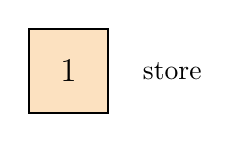
\begin{tikzpicture}
        \node[box, label={[label distance=0.3cm]right:\code{store}}] (N1) {\code{1}};
      \end{tikzpicture}
      \vspace{\fill}
    \end{minipage}
  \end{center}
\end{frame}


\begin{frame}[fragile]
  \frametitle{Debugging Imperative Code}

  \begin{minipage}[t][0.6in][t]{\textwidth}
  First, we enter the call to \code{fact 2}.
  \end{minipage}

  \vspace{10pt}

  \begin{center}
    \begin{minipage}[t][1.7in][t]{0.6\textwidth}
      \vspace{\fill}
      \begin{codeblock}
        fun fact 0 = !store
          `| fact n =`
              ( store := n * (!store);
                fact (n - 1)
              )
      \end{codeblock}
      \vspace{\fill}
    \end{minipage}
    \hfill\vline\hfill
    \begin{minipage}[t][1.7in][t]{0.3\textwidth}
      \centering
      {\hspace{-20pt}\color{gray} \large THE STORE}

      \vspace{\fill}
      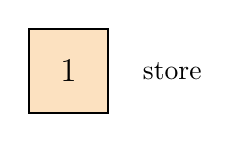
\begin{tikzpicture}
        \node[box, label={[label distance=0.3cm]right:\code{store}}] (N1) {\code{1}};
      \end{tikzpicture}
      \vspace{\fill}
    \end{minipage}
  \end{center}
\end{frame}

\begin{frame}[fragile]
  \frametitle{Debugging Imperative Code}

  \begin{minipage}[t][0.6in][t]{\textwidth}
  The first thing to happen is that we assign \code{store} to the contents
  of \code{store}, multiplied by \code{2}, which is our current value of
  \code{n}.
  \end{minipage}

  \vspace{10pt}

  \begin{center}
    \begin{minipage}[t][1.7in][t]{0.6\textwidth}
      \vspace{\fill}
      \begin{codeblock}
        fun fact 0 = !store
          | fact n =
              ( `store := n * (!store)`;
                fact (n - 1)
              )
      \end{codeblock}
      \vspace{\fill}
    \end{minipage}
    \hfill\vline\hfill
    \begin{minipage}[t][1.7in][t]{0.3\textwidth}
      \centering
      {\hspace{-20pt}\color{gray} \large THE STORE}

      \vspace{\fill}
      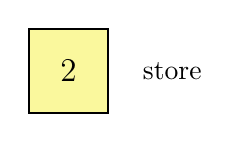
\begin{tikzpicture}
        \node[hlbox, label={[label distance=0.3cm]right:\code{store}}] (N1) {\large \code{2}};
      \end{tikzpicture}
      \vspace{\fill}
    \end{minipage}
  \end{center}
\end{frame}

\begin{frame}[fragile]
  \frametitle{Debugging Imperative Code}

  \begin{minipage}[t][0.6in][t]{\textwidth}
    The next thing we do is that we recurse on \code{n - 1}, which in this case
    is \code{1}.

    \vspace{\fill}

    We won't step through that call explicitly, but suffice to say that it will
    multiply the store by \code{1}, keeping it the same, and then eventually return
    the contents of the store, which is \code{2}.
  \end{minipage}

  \vspace{10pt}

  \begin{center}
    \begin{minipage}[t][1.7in][t]{0.6\textwidth}
      \vspace{\fill}
      \begin{codeblock}
        fun fact 0 = !store
          | fact n =
              ( store := n * (!store);
                `fact (n - 1)`
              )
      \end{codeblock}
      \vspace{\fill}
    \end{minipage}
    \hfill\vline\hfill
    \begin{minipage}[t][1.7in][t]{0.3\textwidth}
      \centering
      {\hspace{-20pt}\color{gray} \large THE STORE}

      \vspace{\fill}
      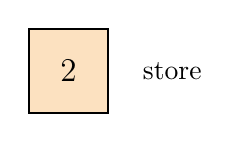
\begin{tikzpicture}
        \node[box, label={[label distance=0.3cm]right:\code{store}}] (N1) {\code{2}};
      \end{tikzpicture}
      \vspace{\fill}
    \end{minipage}
  \end{center}
\end{frame}

\begin{frame}[fragile]
  \frametitle{Debugging Imperative Code}

  \begin{minipage}[t][0.6in][t]{\textwidth}
    But what happens if we immediately then execute \code{fact 2}, again?

    \vspace{\fill}

    Then, we enter the function again...
  \end{minipage}

  \vspace{10pt}

  \begin{center}
    \begin{minipage}[t][1.7in][t]{0.6\textwidth}
      \vspace{\fill}
      \begin{codeblock}
        fun fact 0 = !store
          `| fact n =`
              ( store := n * (!store);
                fact (n - 1)
              )
      \end{codeblock}
      \vspace{\fill}
    \end{minipage}
    \hfill\vline\hfill
    \begin{minipage}[t][1.7in][t]{0.3\textwidth}
      \centering
      {\hspace{-20pt}\color{gray} \large THE STORE}

      \vspace{\fill}
      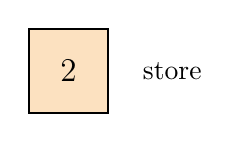
\begin{tikzpicture}
        \node[box, label={[label distance=0.3cm]right:\code{store}}] (N1) {\code{2}};
      \end{tikzpicture}
      \vspace{\fill}
    \end{minipage}
  \end{center}
\end{frame}

\begin{frame}[fragile]
  \frametitle{Debugging Imperative Code}

  \begin{minipage}[t][0.6in][t]{\textwidth}
    ... and multiply what is in the \code{store} by \code{n}, which is \code{2}
  \end{minipage}

  \vspace{10pt}

  \begin{center}
    \begin{minipage}[t][1.7in][t]{0.6\textwidth}
      \vspace{\fill}
      \begin{codeblock}
        fun fact 0 = !store
          | fact n =
              ( `store := n * (!store)`;
                fact (n - 1)
              )
      \end{codeblock}
      \vspace{\fill}
    \end{minipage}
    \hfill\vline\hfill
    \begin{minipage}[t][1.7in][t]{0.3\textwidth}
      \centering
      {\hspace{-20pt}\color{gray} \large THE STORE}

      \vspace{\fill}
      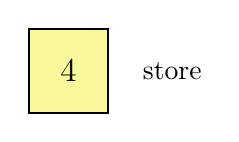
\begin{tikzpicture}
        \node[hlbox, label={[label distance=0.3cm]right:\code{store}}] (N1) {\large \code{4}};
      \end{tikzpicture}
      \vspace{\fill}
    \end{minipage}
  \end{center}
\end{frame}

\begin{frame}[fragile]
  \frametitle{Debugging Imperative Code}

  \begin{minipage}[t][0.6in][t]{\textwidth}
    Then, we recurse finally on \code{fact 1}, which we know will keep the store
    the same and return the contents of the store, which is \code{4}.

    \vspace{\fill}

    So \code{fact 2} $\hookrightarrow$ \code{4}.

    \vspace{\fill}

    Uh oh.
  \end{minipage}

  \vspace{10pt}

  \begin{center}
    \begin{minipage}[t][1.7in][t]{0.6\textwidth}
      \vspace{\fill}
      \begin{codeblock}
        fun fact 0 = !store
          | fact n =
              ( store := n * (!store);
                `fact (n - 1)`
              )
      \end{codeblock}
      \vspace{\fill}
    \end{minipage}
    \hfill\vline\hfill
    \begin{minipage}[t][1.7in][t]{0.3\textwidth}
      \centering
      {\hspace{-20pt}\color{gray} \large THE STORE}

      \vspace{\fill}
      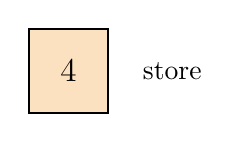
\begin{tikzpicture}
        \node[box, label={[label distance=0.3cm]right:\code{store}}] (N1) {\code{4}};
      \end{tikzpicture}
      \vspace{\fill}
    \end{minipage}
  \end{center}
\end{frame}

\begin{frame}[fragile]
  \frametitle{One \code{ref} to Rue Them All}

  Our problem was that our \code{ref} was too long lasting!

  \vspace{\fill}

  We used the same \code{ref}, which was \textit{never reset}, at any point.

  \pause
  \vspace{\fill}

  In fact, every call to \code{fact} uses that same ref, because we only called
  \code{ref} once, and at the top level, independent of any call to the function
  \code{fact}! This is sure to be a recipe for disaster!

  \pause
  \vspace{\fill}

  A better way to do it would be not to share this memory between different function
  calls. We might prefer to have each call to \code{fact} spawn its own, private
  \code{ref} cell, for use in its calculations.
\end{frame}

\begin{frame}[fragile]
  \frametitle{\code{fact}, re\code{fact}ored}

  Let's rewrite our imperative \code{fact} with that idea in mind.

  \pause
  \vspace{\fill}

  \begin{codeblock}
    fun fact n =
      let
        val store = ref 1
        fun fact' 0 = !store
          | fact' n =
              ( store := n * (!store);
                fact' (n - 1)
              )
      in
        fact' n
      end
  \end{codeblock}
\end{frame}

\begin{frame}[fragile]
  \frametitle{Observational Purity}

  \ptmt

  Now, our \code{fact} function works, because upon entering the function, a
  \code{ref} is allocated. Because it's gated by the function, it's guaranteed
  to be new on each invocation of the function, and thus it is
  safe to be used by the helper function \code{fact'}.

  \pause
  \vspace{\fill}

  In the background, once the \code{fact} function finishes its run, the ref
  cell of \code{store} will be deallocated, and thus not waste any memory.

  \pause
  \vspace{\fill}

  \defBox{}{We say that functions like \code{fact} are \term{observationally pure},
  in that they appear to an outside user to be pure, even though they use side
  effects such as mutability internally.}

  \pause
  \vspace{\fill}

  The key reason why observational purity is OK is because \textit{it is impossible
  to tell from the outside} that the function is not pure! We also call such
  effects used in an observationally pure way a \term{benign effect}.
\end{frame}

\sectionSlide{4}{Aliasing}

\begin{frame}[fragile]
  \frametitle{\code{ref}s as Values}

  Because of the fact that \code{ref} cells are values like any other, we can
  pass them around and bind them to new variables, like any other.

  \pause
  \vspace{\fill}

  We have to be especially careful when we do something like this, however,
  so that we get the correct mental picture for what's happening!

  \pause
  \vspace{\fill}

  For instance, take the following code:

  \begin{codeblock}
    val r1 : int ref     = ref 0
    val r2 : int ref     = r1
    val r3 : int ref ref = ref r1
    val r1 : int ref     = ref 1
    val ()               = r2 := 3
  \end{codeblock}

  \pause
  \vspace{\fill}

  What's going on here?
\end{frame}

\begin{frame}[fragile]
  \frametitle{\code{ref} Chasing}

  \topthing{0.2in}{
    We start off with the empty store, as usual.
  }

  \vspace{10pt}

  \begin{center}
    \begin{minipage}[t][2.1in][t]{0.6\textwidth}
      \vspace{\fill}
      \begin{codeblock}
        val r1 : int ref     = ref 0
        val r2 : int ref     = r1
        val r3 : int ref ref = ref r1
        val r1 : int ref     = ref 1
        val ()               = r2 := 3
      \end{codeblock}
      \vspace{\fill}
    \end{minipage}
    \hfill\vline\hfill
    \begin{minipage}[t][2.1in][t]{0.3\textwidth}
      \centering
      {\hspace{-20pt}\color{gray} \large THE STORE}

      \vspace{\fill}
      \begin{tikzpicture}
        %\node[box, label={[label distance=0.3cm]right:\code{store}}] (N1) {\code{4}};
      \end{tikzpicture}
      \vspace{\fill}
    \end{minipage}
  \end{center}
\end{frame}

\begin{frame}[fragile]
  \frametitle{\code{ref} Chasing}

  \topthing{0.2in}{
    At a call to \code{ref}, we allocate a distinct \code{ref} cell for \code{r1}.
  }

  \vspace{10pt}

  \begin{center}
    \begin{minipage}[t][2.1in][t]{0.6\textwidth}
      \vspace{\fill}
      \begin{codeblock}
        `val r1 : int ref     = ref 0`
        val r2 : int ref     = r1
        val r3 : int ref ref = ref r1
        val r1 : int ref     = ref 1
        val ()               = r2 := 3
      \end{codeblock}
      \vspace{\fill}
    \end{minipage}
    \hfill\vline\hfill
    \begin{minipage}[t][2.1in][t]{0.3\textwidth}
      \centering
      {\hspace{-20pt}\color{gray} \large THE STORE}

      \vspace{\fill}
      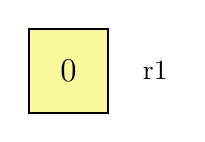
\begin{tikzpicture}
        \node[hlbox, label={[label distance=0.3cm]right:\code{r1}}] (N1) {\large \code{0}};
      \end{tikzpicture}
      \vspace{\fill}
    \end{minipage}
  \end{center}
\end{frame}

\begin{frame}[fragile]
  \frametitle{\code{ref} Chasing}

  \topthing{0.2in}{
    When we bind the value of \code{r1} to \code{r2}, this means that \code{r2}
    now refers to the \textit{same box} as \code{r1}.
  }

  \vspace{10pt}

  \begin{center}
    \begin{minipage}[t][2.1in][t]{0.6\textwidth}
      \vspace{\fill}
      \begin{codeblock}
        val r1 : int ref     = ref 0
        `val r2 : int ref     = r1`
        val r3 : int ref ref = ref r1
        val r1 : int ref     = ref 1
        val ()               = r2 := 3
      \end{codeblock}
      \vspace{\fill}
    \end{minipage}
    \hfill\vline\hfill
    \begin{minipage}[t][2.1in][t]{0.3\textwidth}
      \centering
      {\hspace{-20pt}\color{gray} \large THE STORE}

      \vspace{\fill}
      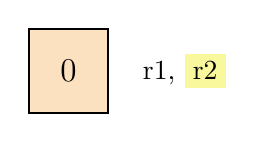
\begin{tikzpicture}
        \node[box, label={[label distance=0.3cm]right:\code{r1}, \colorbox{highlightColor}{\code{r2}}}] (N1) {\code{0}};
      \end{tikzpicture}
      \vspace{\fill}
    \end{minipage}
  \end{center}
\end{frame}

\begin{frame}[fragile]
  \frametitle{\code{ref} Chasing}

  \topthing{0.2in}{
    We then allocate a box which itself \textit{points to} the box of \code{r1},
    which we denote via a box with an arrow directed at the box of \code{r1}.
  }

  \vspace{10pt}

  \begin{center}
    \begin{minipage}[t][2.1in][t]{0.6\textwidth}
      \vspace{\fill}
      \begin{codeblock}
        val r1 : int ref     = ref 0
        val r2 : int ref     = r1
        `val r3 : int ref ref = ref r1`
        val r1 : int ref     = ref 1
        val ()               = r2 := 3
      \end{codeblock}
      \vspace{\fill}
    \end{minipage}
    \hfill\vline\hfill
    \begin{minipage}[t][2.1in][t]{0.3\textwidth}
      \centering
      {\hspace{-20pt}\color{gray} \large THE STORE}

      \vspace{\fill}
      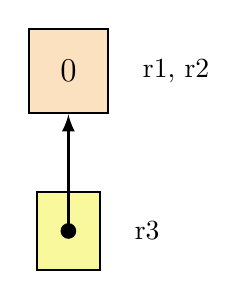
\begin{tikzpicture}
        \node[box, label={[label distance=0.3cm]right:\code{r1}, \code{r2}}] (N1) {\code{0}};
        \node[hlbox, label={[label distance=0.3cm]right:\code{r3}}, below of=N1, node distance=0.8in] (N2) {};
        \draw[-latex, line width=0.4mm] (N2.center) -- node[pos=0, circle, fill=black, inner sep=2pt] {} (N1);
      \end{tikzpicture}
      \vspace{\fill}
    \end{minipage}
  \end{center}
\end{frame}

\begin{frame}[fragile]
  \frametitle{\code{ref} Chasing}

  \topthing{0.2in}{
    We then re-bind \code{r1} to a different \code{ref} cell. This affects neither
    \code{r2}, which has the same value, nor what \code{r3} is pointing at!
  }

  \vspace{10pt}

  \begin{center}
    \begin{minipage}[t][2.1in][t]{0.6\textwidth}
      \vspace{\fill}
      \begin{codeblock}
        val r1 : int ref     = ref 0
        val r2 : int ref     = r1
        val r3 : int ref ref = ref r1
        `val r1 : int ref     = ref 1`
        val ()               = r2 := 3
      \end{codeblock}
      \vspace{\fill}
    \end{minipage}
    \hfill\vline\hfill
    \begin{minipage}[t][2.1in][t]{0.3\textwidth}
      \centering
      {\hspace{-20pt}\color{gray} \large THE STORE}

      \vspace{\fill}
      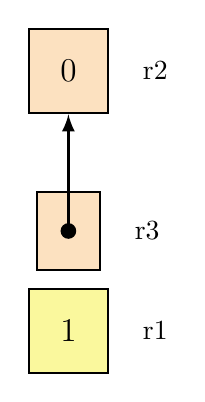
\begin{tikzpicture}
        \node[box, label={[label distance=0.3cm]right:\code{r2}}] (N1) {\code{0}};
        \node[box, label={[label distance=0.3cm]right:\code{r3}}, below of=N1, node distance=0.8in] (N2) {};
        \node[hlbox, label={[label distance=0.3cm]right:\code{r1}}, below of=N2, node distance=0.5in] (N3) {\large \code{1}};
        \draw[-latex, line width=0.4mm] (N2.center) -- node[pos=0, circle, fill=black, inner sep=2pt] {} (N1);
      \end{tikzpicture}
      \vspace{\fill}
    \end{minipage}
  \end{center}
\end{frame}

\begin{frame}[fragile]
  \frametitle{\code{ref} Chasing}

  \topthing{0.2in}{
    We can then update the contents of \code{r2}'s box to \code{3},
    which is independent of \code{r1}'s new box, but affects \code{r3}
    indirectly.
  }

  \vspace{10pt}

  \begin{center}
    \begin{minipage}[t][2.1in][t]{0.6\textwidth}
      \vspace{\fill}
      \begin{codeblock}
        val r1 : int ref     = ref 0
        val r2 : int ref     = r1
        val r3 : int ref ref = ref r1
        val r1 : int ref     = ref 1
        `val ()               = r2 := 3`
      \end{codeblock}
      \vspace{\fill}
    \end{minipage}
    \hfill\vline\hfill
    \begin{minipage}[t][2.1in][t]{0.3\textwidth}
      \centering
      {\hspace{-20pt}\color{gray} \large THE STORE}

      \vspace{\fill}
      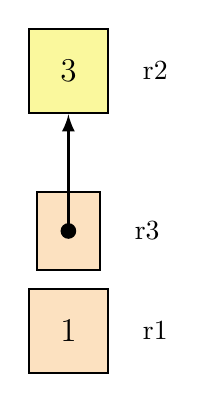
\begin{tikzpicture}
        \node[hlbox, label={[label distance=0.3cm]right:\code{r2}}] (N1) {\large \code{3}};
        \node[box, label={[label distance=0.3cm]right:\code{r3}}, below of=N1, node distance=0.8in] (N2) {};
        \node[box, label={[label distance=0.3cm]right:\code{r1}}, below of=N2, node distance=0.5in] (N3) {\code{1}};
        \draw[-latex, line width=0.4mm] (N2.center) -- node[pos=0, circle, fill=black, inner sep=2pt] {} (N1);
      \end{tikzpicture}
      \vspace{\fill}
    \end{minipage}
  \end{center}
\end{frame}

\begin{frame}[fragile]
  \frametitle{Pointers, Pointers}

  Such is the pointer-chasing logic common to imperative programming.

  \pause
  \vspace{\fill}

  The diagram is made easier to understand if you cognize the fact that, since
  there are three calls to \code{ref}, there must be three ref cells allocated
  over the course of the trace.

  \pause
  \vspace{\fill}

  In addition, it is impossible to change the contents of a box without a
  call to \code{:=}! So be on the lookout for cheap ways to verify your
  thinking, when thinking about \code{ref}s and pointers.

  \pause
  \vspace{\fill}

  Remember, there's nothing special about boxes. They can be bound to other
  variables at will.

  \vspace{\fill}

  \noteBox{\, One might say, \textit{boxes are values}.\footnote{And pointers are boxes. Let transitivity take it from here.}}
\end{frame}

\begin{frame}[fragile]
  \frametitle{\code{ref}s within \code{ref}s}

  As we saw in the previous example, we can have \code{ref}s which point
  to other \code{ref}s.

  \pause
  \vspace{\fill}

  In conjunction with recursive types, this lets us define arbitrary powerful
  imperative structures. For instance, we could define a type for imperative
  linked lists:

  \pause
  \vspace{\fill}

  \begin{codeblock}
    (* I used the term "llist" last lecture, unfortunately *)
    datatype 'a mut_list = Nil | Cons of 'a * 'a mut_list ref
  \end{codeblock}

  \pause
  \vspace{\fill}

  Notably, such a type can have cycles, which is not something you can have
  with ordinary recursive datatypes! For instance:

  \begin{codeblock}
    val r : int mut_list ref = ref Nil
    val l = Cons (1, r)
    val () = r := l
  \end{codeblock}
\end{frame}

\begin{frame}[fragile]
  \frametitle{A Circular Picture}

  \topthing{0.2in}{
    Let's explore exactly what's going on here. We start off with the empty store.
  }

  \vspace{10pt}

  \begin{center}
    \begin{minipage}[t][2.1in][t]{0.55\textwidth}
      \vspace{\fill}
      \small
      \begin{codeblock}
        val r : int mut_list ref = ref Nil
        val l = Cons (1, r)
        val () = r := l
      \end{codeblock}
      \vspace{\fill}
    \end{minipage}
    \hfill\vline\hfill
    \begin{minipage}[t][2.1in][t]{0.35\textwidth}
      \centering
      {\hspace{-20pt}\color{gray} \large THE STORE}

      \vspace{\fill}
      \begin{tikzpicture}
      \end{tikzpicture}
      \vspace{\fill}
    \end{minipage}
  \end{center}
\end{frame}

\begin{frame}[fragile]
  \frametitle{A Circular Picture}

  \topthing{0.2in}{
    Then, we allocate a single reference cell containing the empty \code{mut_list}.
  }

  \vspace{10pt}

  \begin{center}
    \begin{minipage}[t][2.1in][t]{0.55\textwidth}
      \vspace{\fill}
      \small
      \begin{codeblock}
        `val r : int mut_list ref = ref Nil`
        val l = Cons (1, r)
        val () = r := l
      \end{codeblock}
      \vspace{\fill}
    \end{minipage}
    \hfill\vline\hfill
    \begin{minipage}[t][2.1in][t]{0.35\textwidth}
      \centering
      {\hspace{-20pt}\color{gray} \large THE STORE}

      \vspace{\fill}
      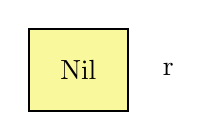
\begin{tikzpicture}
        \node[hlbox, label={[label distance=0.3cm]right:\code{r}}] (N1) {\code{Nil}};
      \end{tikzpicture}
      \vspace{\fill}
    \end{minipage}
  \end{center}
\end{frame}

\begin{frame}[fragile]
  \frametitle{A Circular Picture}

  \topthing{0.2in}{
    We then bind the value of \code{Cons (1, r)} to \code{l}.
  }

  \vspace{10pt}

  \begin{center}
    \begin{minipage}[t][2.1in][t]{0.55\textwidth}
      \vspace{\fill}
      \small
      \begin{codeblock}
        val r : int mut_list ref = ref Nil
        `val l = Cons (1, r)`
        val () = r := l
      \end{codeblock}
      \vspace{\fill}
    \end{minipage}
    \hfill\vline\hfill
    \begin{minipage}[t][2.1in][t]{0.35\textwidth}
      \centering
      {\hspace{-20pt}\color{gray} \large THE STORE}

      \vspace{\fill}
      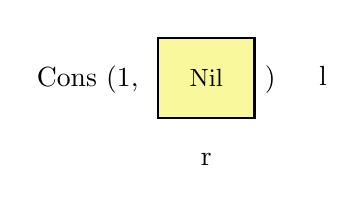
\begin{tikzpicture}
        \node[label={[yshift=0.38cm, label distance=0.3cm]right:\code{l}}] (N2) {
          \code{Cons (1, }
          \tikz[baseline, anchor=base] \node[hlbox, label={[label distance=0.3cm]below:\code{r}}] (N1) {\small \code{Nil}};
          \code{)}
        };
      \end{tikzpicture}
      \vspace{\fill}
    \end{minipage}
  \end{center}
\end{frame}

\begin{frame}[fragile]
  \frametitle{A Circular Picture}

  \topthing{0.2in}{
    Here's where the "contains" analogy becomes imperfect. But basically, we cause
    \code{r} to now point to the \code{Cons} node, which is perfectly legal.
  }

  \vspace{10pt}

  \begin{center}
    \begin{minipage}[t][2.1in][t]{0.55\textwidth}
      \vspace{\fill}
      \small
      \begin{codeblock}
        val r : int mut_list ref = ref Nil
        val l = Cons (1, r)
        `val () = r := l`
      \end{codeblock}
      \vspace{\fill}
    \end{minipage}
    \hfill\vline\hfill
    \begin{minipage}[t][2.1in][t]{0.35\textwidth}
      \centering
      {\hspace{-20pt}\color{gray} \large THE STORE}

      \vspace{\fill}
      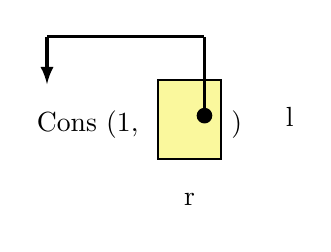
\begin{tikzpicture}
        \node[label={[yshift=0.38cm, label distance=0.3cm]right:\code{l}}] (N2) {
          \code{Cons (1, }
          \tikz[baseline, anchor=base] \node[hlbox, yshift=0.15cm, label={[label distance=0.3cm]below:\code{r}}] (N1) {};
          \code{)}
        };
        \node[right of=N1, node distance=0.825cm, yshift=0.25cm] (N4) {};
        \node[above of=N4, node distance=1cm] (N5) {};
        \node[left of=N5, node distance=2cm] (N6) {};
        \node[below of=N6, node distance=0.6cm] (N7) {};
        \draw[line width=0.4mm] (N4.center) -- node[pos=0, circle, fill=black, inner sep=2pt] {} (N5.center);
        \draw[line width=0.4mm] (N5.center) -- (N6.center);
        \draw[-latex, line width=0.4mm] (N6.center) -- (N7.center);
      \end{tikzpicture}
      \vspace{\fill}
    \end{minipage}
  \end{center}
\end{frame}

\sectionSlide{5}{Applications of Mutability (Bonus)}

\begin{frame}[fragile]
  \frametitle{Mutability and Parallelism}

  Mutability is generally problematic, but it doesn't need to be avoided at all
  costs.

  \pause
  \vspace{\fill}

  One thing to realize about mutability is that it inherently causes problems
  with parallelism. One nice property we talked about on the first day was
  the ability to reason about components of functional programs independently --
  this is because those components must always evaluate the same, in the absence
  of effects.

  \pause
  \vspace{\fill}

  Mutability \textit{can} be safe in a deterministic environment, but it becomes
  much more difficult to control when running a parallel program.

  \vspace{\fill}

  \begin{center}
    \begin{tabular}{ c|c|c }
     & Sequential & Parallel \\
    \hline & \\[-1.5ex]
    Immutable & {\color{green!70!black}safe} & {\color{green!70!black}safe} \\ [0.5ex]
    \hline & \\[-1.5ex]
    Mutable & {\color{orange} harder, but possible} & {\color{red} no man's land}
    \end{tabular}
  \end{center}
\end{frame}

\begin{frame}[fragile]
  \frametitle{Mutability in Practice}

  There are some common techniques that can be used in a functional setting
  with \code{ref} cells, however. These are generally more innocent, and have
  less to do with persistent usage of mutable state, as more occasional
  usages of mutability as a labor-saving device.

  \pause
  \vspace{\fill}

  Remember, purity is a trap. We don't serve immutability -- immutability and
  mutability serve us.
\end{frame}

\begin{frame}[fragile]
  \frametitle{Mutability Technique: Fresh IDs}

  We can use \code{ref} cells to generate fresh integers (or \textit{temps}), that
  are guaranteed to be unique across a single program's lifetime.

  \pause
  \vspace{\fill}

  \customBox{Use Cases}{\, Unique identifiers for each node in a graph, each
  person in a database, each variable in a program, each transaction in a
  system.}

  \pause
  \vspace{\fill}

  We do this by simply using an \code{int ref} which we increment every time
  we get a new ID.

  \pause
  \vspace{\fill}

  \begin{codeblock}
    val id_store = ref 0

    fun fresh () =
      ( id_store := 1 + (!id_store);
        !id_store
      )
  \end{codeblock}
\end{frame}

\begin{frame}[fragile]
  \frametitle{Mutability Technique: Fresh IDs}

  These IDs are known to be \code{int}s, though, so it's possible we might
  accidentally do arithmetic on them and get a different ID when we didn't
  mean to.

  \pause
  \vspace{\fill}

  We can use this technique in conjunction with opaque ascription to prevent
  that!

  \pause
  \vspace{\fill}

  \begin{codeblock}
    structure UNIQUE_ID =
      sig
        (* an abstract type of fresh identifiers *)
        type t

        val fresh : unit -> t

        (* need an equality function, or the type is useless *)
        val eq : t * t -> bool
      end
  \end{codeblock}
\end{frame}

\begin{frame}[fragile]
  \frametitle{Mutability Technique: Fresh IDs}

  Then, we just opaquely ascribe to the above signature to be able to
  make sure users can only construct values of type \code{UniqueId.t}
  through the structure.

  \pause
  \vspace{\fill}

  \begin{codeblock}
    structure UniqueId :> UNIQUE_ID =
      struct
        (* internally an `int`, but users don't know that! *)
        type t = int

        val id_store = ref 0

        fun fresh () =
          ( id_store := 1 + (!id_store);
            !id_store
          )
        val eq = (op=)
    end
  \end{codeblock}
\end{frame}

\begin{frame}[fragile]
  \frametitle{Mutability Technique: Hooks}

  Suppose that you want to be able to dynamically load a given function,
  but you don't know what it is, necessarily, and you also can't write the
  function right now.

  \pause
  \vspace{\fill}

  There's lots of reasons why you might want to be able to use a function,
  but you can't write it in the file you need it in. This could be due to
  compilation dependencies, types you need being defined elsewhere, or just
  general program logic living somewhere else.

  \pause
  \vspace{\fill}

  You can make your dependencies run \textit{backwards} by providing a
  \code{ref} cell that will \textit{eventually} contain the function you
  want, and then \term{backpatching} it at a later point, filling in
  the cell before you use it.
\end{frame}

\begin{frame}[fragile]
  \frametitle{Mutability Technique: Hooks}

  \defBox{\, A \term{hook} is a \code{ref} of type \code{t option ref}, where
  \code{t} is usually a function type. It starts off as \code{NONE}, and then
  at a later point is filled in to be \code{SOME v}, downstream.}

  \pause
  \vspace{\fill}

  \begin{codeblock}
    val function_i_need_but_dont_have_hook :
      (int -> int) ref = ref NONE
  \end{codeblock}

  \pause
  \vspace{\fill}

  Then, several files downstream, we might write:
  \begin{codeblock}
    fun f x = (* ... *)

    val _ = function_i_need_but_dont_have_hook := SOME f
  \end{codeblock}

  \pause
  \vspace{\fill}

  This fills in the hook, usually before we even get the chance to use it, so
  we cover our use cases.

  \pause
  \vspace{\fill}

  This is also a useful way to make a piece of software's behavior easily
  changeable via an outside consumer, by having users have the option to
  set the hook.
\end{frame}

\begin{frame}[fragile]
  \frametitle{Mutability Technique: Global Settings}

  Another classic technique is to have a \code{ref} which mediates some
  setting which governs the program's entire runtime.

  \pause
  \vspace{\fill}

  This is better than explicitly passing that value down through every place where
  it needs to be used, which would cause an immense amount of bloat in the program!

  \pause
  \vspace{\fill}

  \begin{codeblock}
    fun initialize_api is_verbose () =
      let
        val () = if is_verbose then
                   print "Initializing API...\n"
                 else ()
      in
        (* ... *)
      end
  \end{codeblock}
\end{frame}

\begin{frame}[fragile]
  \frametitle{Mutability Technique: Global Settings}

  Here, we kill the explicit argument \code{is_verbose}, which would
  presumably need to be passed through approximately fifty billion functions,
  and instead reference a \code{bool ref} called \code{is_verbose}, which is
  set someplace else.

  \pause
  \vspace{\fill}

  \begin{codeblock}
    fun initialize_api & & () =
      let
        val () = if `!is_verbose` then
                   print "Initializing API...\n"
                 else ()
      in
        (* ... *)
      end
  \end{codeblock}

  \pause
  \vspace{\fill}

  This is safer to do, because we generally only will set this property once
  per invocation of a program.
\end{frame}

% \begin{frame}[plain]
% 	\begin{center} Thank you! \end{center}

% 	\begin{center}
%     {\color{blue} \href{https://docs.google.com/forms/d/e/1FAIpQLSf6J6RjAweoMZwnYg5yCL-9_6rlatT5qCrlREywptoCR0Y9Bw/viewform?usp=sf_link}{Post-lecture survey:}} \\
%     \vspace{5pt}
%     \includegraphics[scale=0.035]{qr_july20} \\
%     \vspace{5pt}
%     And the House Quiz winner is...
%   \end{center}
% \end{frame}

\thankyou


\end{document}
